\subsection{Design}

An initial design meeting was held to agree overall technical approach.
Reference is made to Appendix \ref{appendix:design_meeting} for further details.
Since this meeting, the design evolved as the team got more familiar with the design challenges.

This section communicates the final design.
Where possible, the team implemented common design patterns in an effort to reduce coupling and to follow best-practices.
Overall architecture makes use of the MVC pattern, applied per Figure \ref{figure:system_architecture}.

\begin{center}
	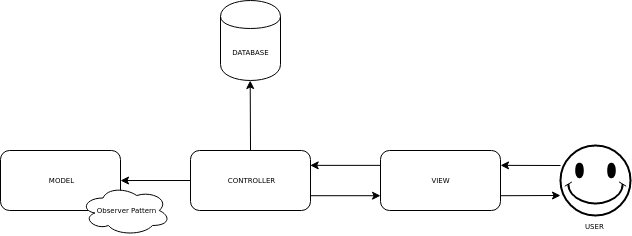
\includegraphics[scale=0.7]{system_architecture}
	\captionof{figure}{System Architecture}
	\label{figure:system_architecture}
\end{center}

The model and database components were designed to be used by either the command line or online modes of the system:

\begin{itemize}
	\item Model (\texttt{package model}, see Figure \ref{figure:model_uml} for UML):
	\begin{itemize}
		\item Encapsulate game actions and game state.
		\item Be agnostic to the implementation of other parts of the system. Apply the Observer Pattern to eliminate any need for the model to be aware of external components, reducing coupling. Passively notify interested parties of changes to game state.
		\item Provide a set of public methods to trigger key game actions (Facade Pattern) (\texttt{GameAPI.java}).
		\item Provide a Immutable Parameter Object to extract a snapshot of key game data from within the model, allowing a single ``info'' object to passed to other parts of the system (\texttt{GameInfo.java}).
	\end{itemize}

	\item Database (\texttt{package persistence}, see Figure \ref{figure:persistence_uml} for UML):
	\begin{itemize}
		\item Provide a set of public methods to write key game information to a persistent database.
	\end{itemize}
\end{itemize}

A specific controller and views were created for command line mode:

\begin{itemize}
	\item Controller (\texttt{package commandline}, see Figure \ref{figure:commandline_uml} for UML):
	\begin{itemize}
		\item Provide game management and logical flow, specific to the command line implementation .
		\item Serve views to user, and trigger necessary game actions.
		\item Trigger game events based on game state (via Observer).
		\item Limit coupling with model by calling \texttt{GameAPI.java} methods only.
	\end{itemize}

	\item View(s) (\texttt{package commandline}, see Figure \ref{figure:commandline_uml} for UML):
	\begin{itemize}
		\item Provide command line output and facilities to retrieve user input, specific to the command line implementation.
		\item Limit coupling by communicating only with the controller.
	\end{itemize}
\end{itemize}

For online mode:

\begin{itemize}
	\item Controller (\texttt{package online}), see Figure \ref{figure:online_uml} for UML):
	\begin{itemize}
		\item Provide game management and logical flow, specific to the online implementation.
		\item Provide APIs for the user to interact with the Game logic via the web page views.
		\item Trigger game events based on user interaction via web pages (i.e. API calls).
		\item Limit coupling with model by calling \texttt{GameAPI.java} methods only.
	\end{itemize}

	\item View(s) (\texttt{package online}), see Figure \ref{figure:online_uml} for UML):
	\begin{itemize}
		\item Provide output and receive user input via (.ftl) web pages specific for the online implementation.
		\item Coupling limited by freeing the web pages from interacting with the Game logic.
	\end{itemize}
\end{itemize}

The interaction between all packages is captured in Figure \ref{figure:full_uml}. 
The native image is also provided with the team .zip submission for readability.

\newpage
\begin{center}
	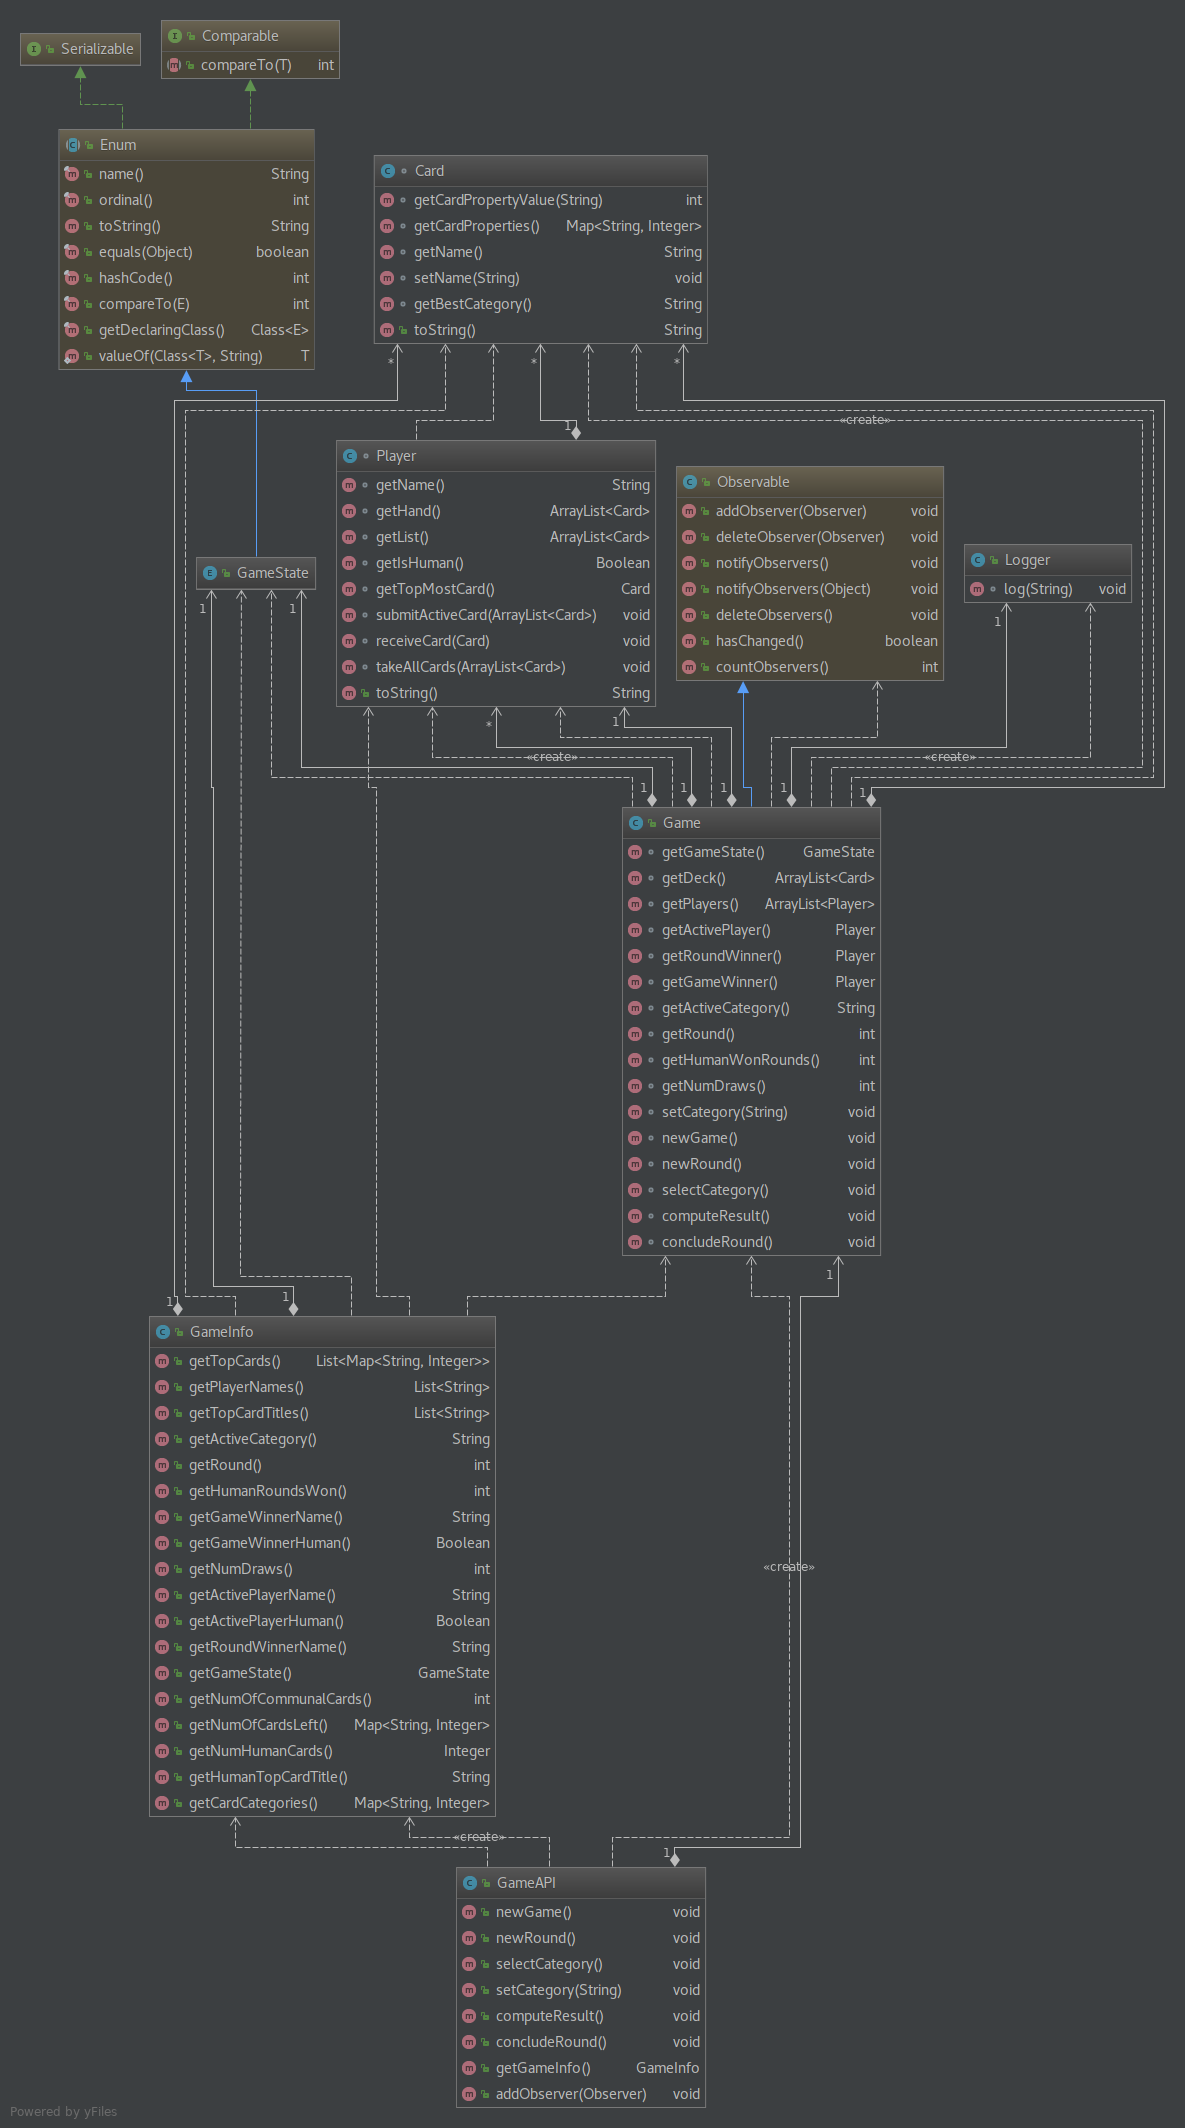
\includegraphics[scale=0.29]{final_UML_model_package}
	\captionof{figure}{Model Package UML (Package Visibility)}
	\label{figure:model_uml}
\end{center}

\begin{center}
	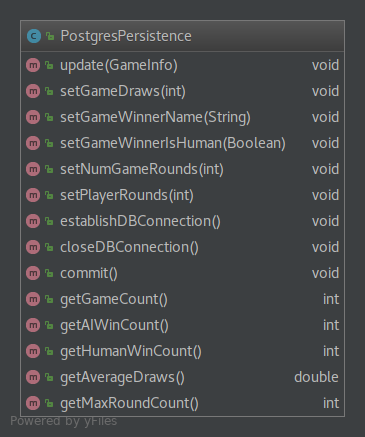
\includegraphics[scale=0.4]{final_UML_persistence_package}
	\captionof{figure}{Persistence Package UML (Package Visibility)}
	\label{figure:persistence_uml}
\end{center}

\begin{center}
	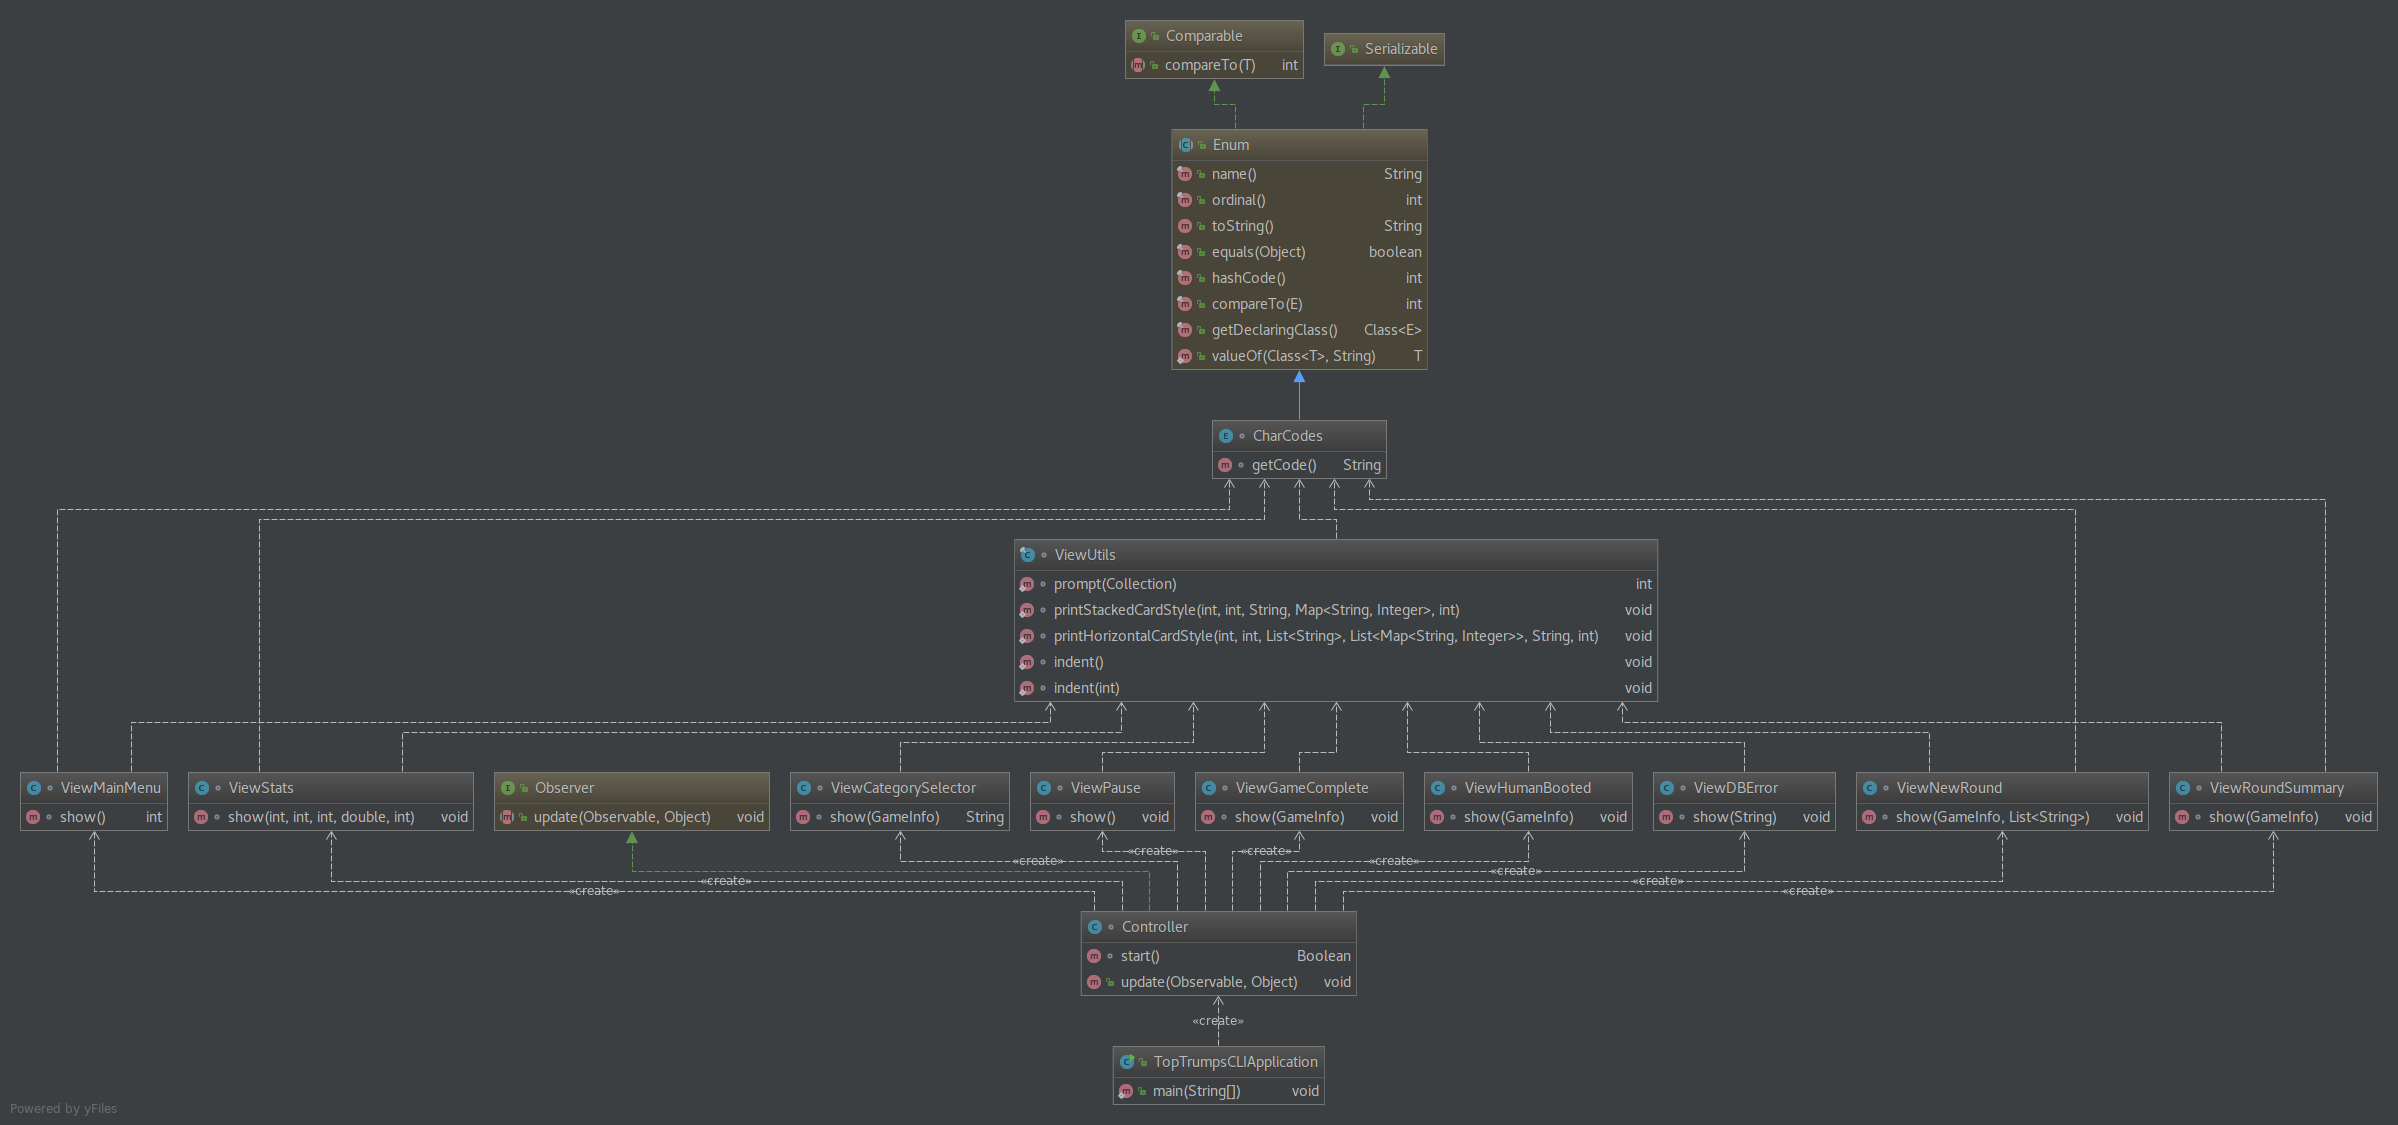
\includegraphics[width=\textwidth]{final_UML_commandline_package}
	\captionof{figure}{Commandline Package UML (Package Visibility)}
	\label{figure:commandline_uml}
\end{center}

\begin{center}
	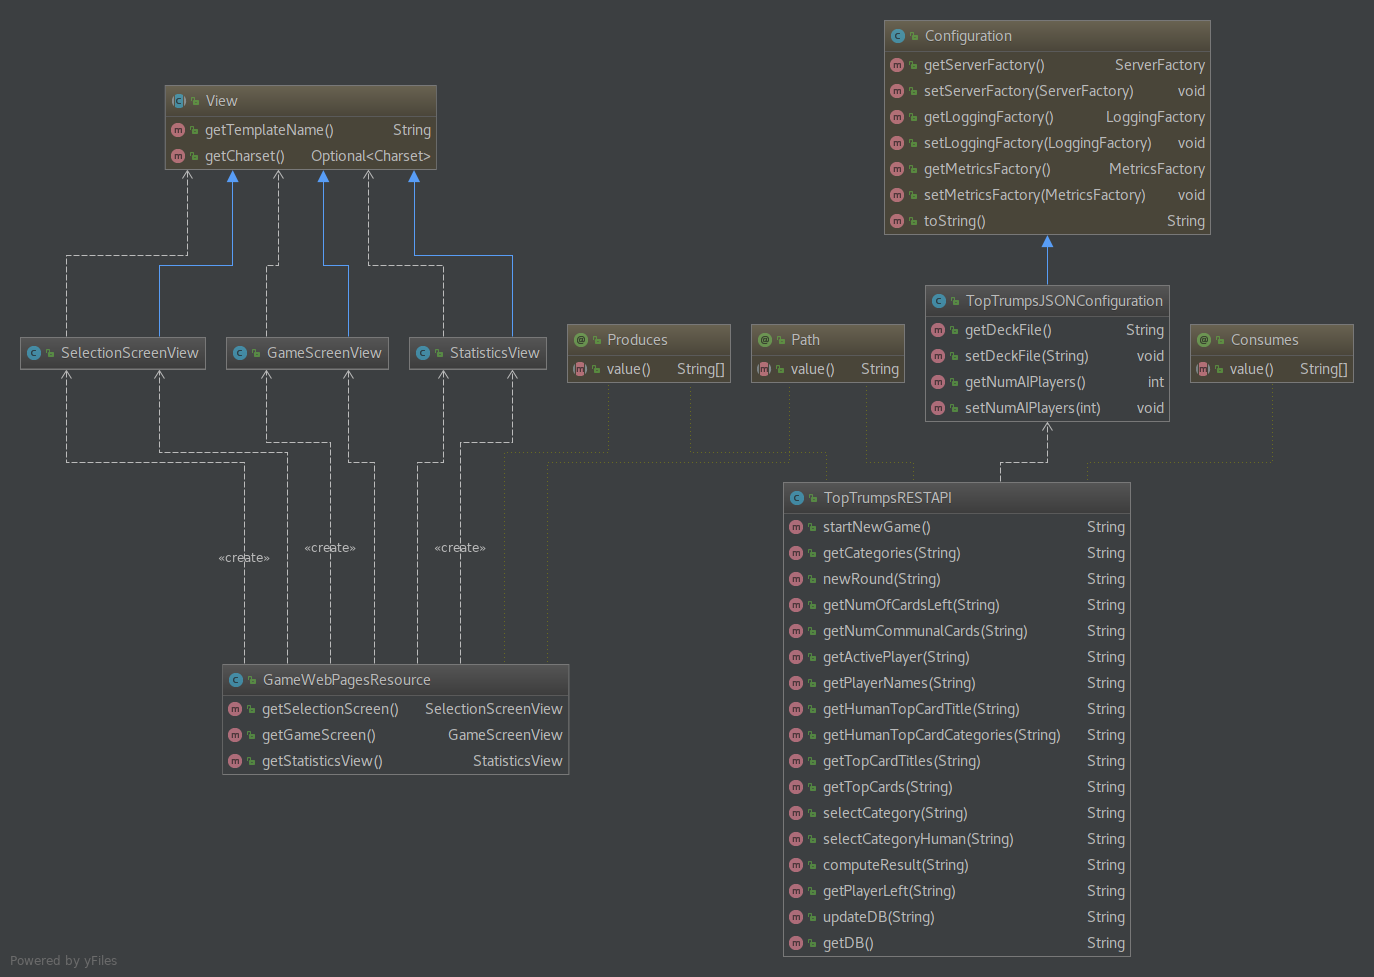
\includegraphics[width=\textwidth]{final_UML_online_package}
	\captionof{figure}{Online Package UML (Package Visibility)}
	\label{figure:online_uml}
\end{center}

\begin{center}
	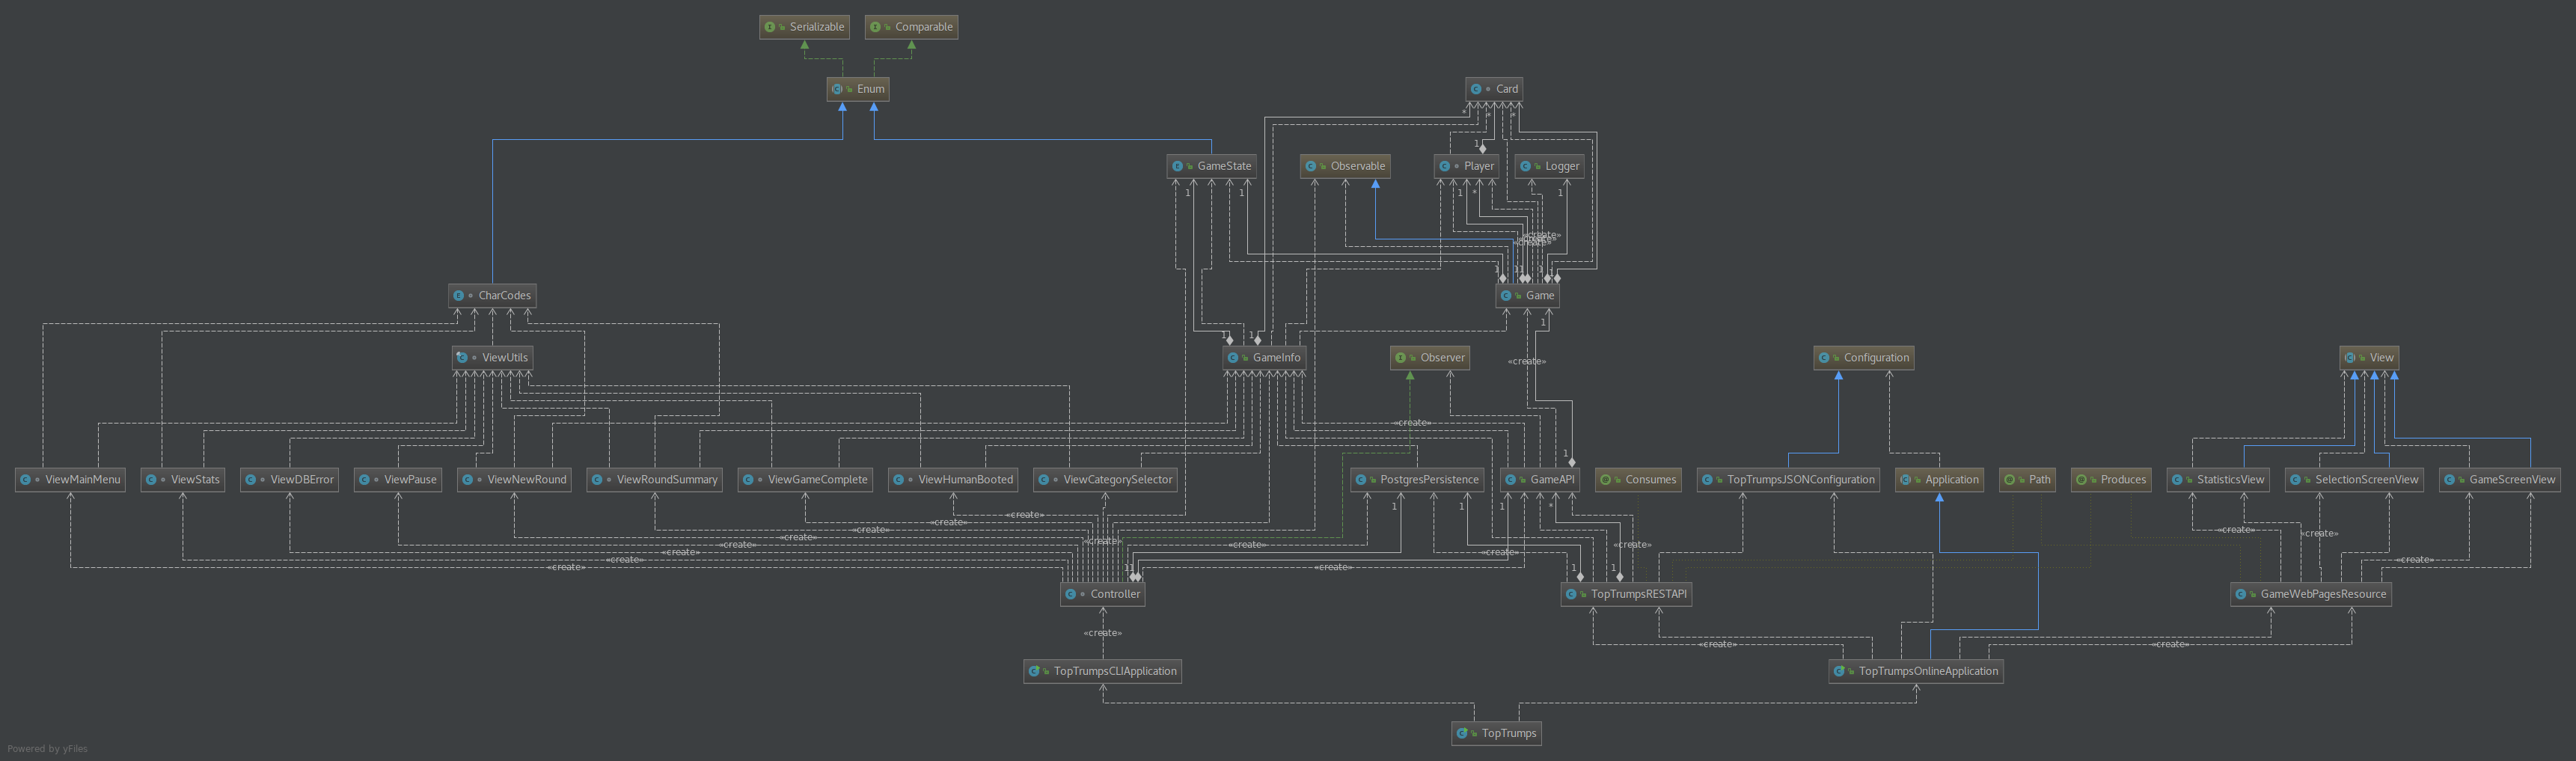
\includegraphics[scale=0.19, angle=90]{final_uml_full}
	\captionof{figure}{Full System UML.}
	\label{figure:full_uml}
\end{center}